\documentclass[border=12pt]{standalone}
\usepackage{xcolor}
\usepackage{tikz}
\usetikzlibrary{arrows.meta,patterns,bending}
\def\wall{
    \fill [fill=black!50,draw=violet,line width=1pt] (1,-.5) rectangle (2,.5);
    \pattern [pattern=bricks] (1,-.5) rectangle (2,.5);
}
\begin{document}
    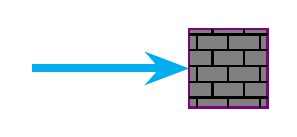
\begin{tikzpicture}
        \draw [cyan,-Stealth,line width=1mm] (-1,0) -- (1,0);
        \wall
    \end{tikzpicture}

    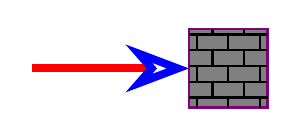
\begin{tikzpicture}
        \draw [red,line width=1mm,-{Stealth[length=.8cm,open,blue]}] (-1,0) -- (1,0); 
        \wall
        %出现 path shortened TiKZ 问题
        %箭头指向出现 tip end 问题
    \end{tikzpicture}

    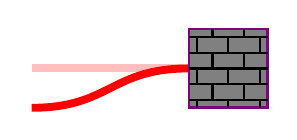
\begin{tikzpicture}
        \draw [red!25,line width=1mm] (-1,0) -- (1,0);
        \draw [red,line width=1mm] (-1,-.5) .. controls (0,-.5) and (0,0) .. (1,0);
        \wall
    \end{tikzpicture}

    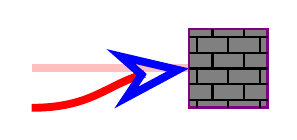
\begin{tikzpicture}
        \draw [red!25,line width=1mm] (-1,0) -- (1,0);
        \draw [red,line width=1mm,-{Stealth[length=1cm,open,blue]}] 
        (-1,-.5) .. controls (0,-.5) and (0,0) .. (1,0);
        \wall
    \end{tikzpicture}

    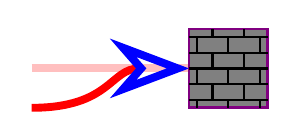
\begin{tikzpicture}
        \draw [red!25,line width=1mm] (-1,0) -- (1,0);
        \draw [red,line width=1mm,-{Stealth[length=1cm,open,blue,quick]}] %使用quick选项微调
        (-1,-.5) .. controls (0,-.5) and (0,0) .. (1,0);
        \wall
    \end{tikzpicture}

    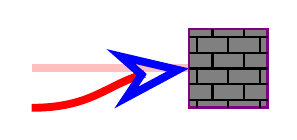
\begin{tikzpicture}
        \draw [red!25,line width=1mm] (-1,0) -- (1,0);
        \draw [red,line width=1mm,-{Stealth[length=1cm,open,blue,flex]}] % 使用bending提供的flex选项微调尾部位置
        (-1,-.5) .. controls (0,-.5) and (0,0) .. (1,0);
        \wall
    \end{tikzpicture}

    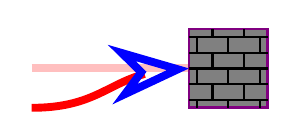
\begin{tikzpicture}
        \draw [red!25,line width=1mm] (-1,0) -- (1,0);
        \draw [red,line width=1mm,-{Stealth[length=1cm,open,blue,flex=.6]}] % 使用bending提供的flex选项微调尾部位置
        (-1,-.5) .. controls (0,-.5) and (0,0) .. (1,0);
        \wall
    \end{tikzpicture}

    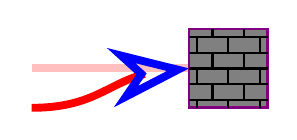
\begin{tikzpicture}
        \draw [red!25,line width=1mm] (-1,0) -- (1,0);
        \draw [red,line width=1mm,-{Stealth[length=1cm,open,blue,flex'=.6]}] % 使用bending提供的flex选项微调尾部位置
        (-1,-.5) .. controls (0,-.5) and (0,0) .. (1,0);
        \wall
    \end{tikzpicture}

    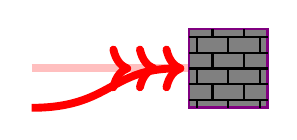
\begin{tikzpicture}
        \draw [red!25,line width=1mm] (-1,0) -- (1,0);
        \draw [red,line width=1mm,-{[quick,sep]>>>}] 
        (-1,-.5) .. controls (0,-.5) and (0,0) .. (1,0);
        \wall % 多箭头单纯使用 quick 选项效果不满意
    \end{tikzpicture}

    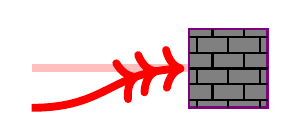
\begin{tikzpicture}
        \draw [red!25,line width=1mm] (-1,0) -- (1,0);
        \draw [red,line width=1mm,-{[flex,sep]>>>}] 
        (-1,-.5) .. controls (0,-.5) and (0,0) .. (1,0);
        \wall % 多箭头单纯使用 quick 选项效果不满意
    \end{tikzpicture}

    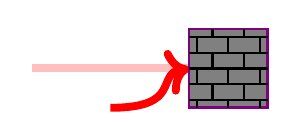
\begin{tikzpicture}
        \draw [red!25,line width=1mm] (-1,0) -- (1,0);
        \draw [red,line width=1mm,-{Computer Modern Rightarrow[flex'=.75]}]
        (0,-.5) .. controls (1,-.5) and (0.5,0) .. (1,0);
        \wall
    \end{tikzpicture}

    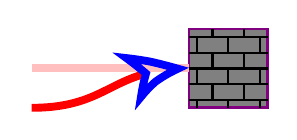
\begin{tikzpicture}
        \wall
        \draw [red!25,line width=1mm] (-1,0) -- (1,0);
        \draw [red,line width=1mm,-{Stealth[length=1cm,bend,blue,open]}]
        (-1,-.5) .. controls (0,-.5) and (0,0) .. (1,0);
    \end{tikzpicture}

    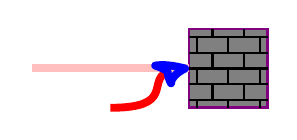
\begin{tikzpicture}
        \wall
        \draw [red!25,line width=1mm] (-1,0) -- (1,0);
        \draw [red,line width=1mm,-{Stealth[bend,round,length=20pt,blue,open]}]
        (0,-.5) .. controls (1,-.5) and (0.25,0) .. (1,0);
    \end{tikzpicture}

\end{document}
